% !TEX root = ../Vorlage_DA.tex
%	########################################################
% 							Arbeitstitel
%	########################################################


%	--------------------------------------------------------
% 	Überschrift, Inhaltsverzeichnis
%	--------------------------------------------------------
\chapter*{Thema: \newline \htlArbeitsthema }



%	--------------------------------------------------------
% 	Bearbeiter
%	--------------------------------------------------------
\section*{Subthemen und Bearbeiter:}


\textbf{Umweltdatenerfassung}\\ 
Andreas Herz, 5BHELS\\
\emph{Betreuer:} Dipl.-Ing. Roland Sageder\\[2ex] 
%
\textbf{Basisstation}\\ 
Andreas Herz, 5BHELS\\
\emph{Betreuer:} Dipl.-Ing. Roland Sageder\\[2ex] 




%--------------------------------------------------------------------------------
%  Vorgeschriebene Dokumentationsseiten
%--------------------------------------------------------------------------------

\pagebreak
\thispagestyle{empty}
\newgeometry{top=2cm, bottom=1.5cm}

\begin{minipage}[c]{0.20\linewidth}
\includegraphics[width=0.8\linewidth]{media/images/htl_c_cmyk_rein}
\end{minipage}
\begin{minipage}[c]{0.6\linewidth}
\begin{center}
{\bfseries\sffamily\large Höhere  technische  Bundeslehranstalt\\
und  Bundesfachschule  Braunau\\
Elektronik und Technische Informatik\\
{\normalsize Schulautonomer Schwerpunkt Communications} }
\end{center}
\end{minipage}
\begin{minipage}[c]{0.2\linewidth}
\hfill \includegraphics[width=0.8\linewidth]{media/images/htl-bildung-mit-zukunft}
\end{minipage}\\

\vspace{1em}
\begin{center}
\bfseries\sffamily\Large
DIPLOMARBEIT DOKUMENTATION
\end{center}
\vspace{1ex}

\renewcommand{\arraystretch}{2}
\begin{tabularx}{1\textwidth}{ p{3.5cm} X }

\textbf{Verfasser/innen} & 
Andreas Herz \\

\textbf{Jahrgang\linebreak Schuljahr} & 
5BHELS 2018/2019 \\

\textbf{\mbox{Thema der} \mbox{Diplomarbeit}} & 
\htlArbeitsthema \\

\textbf{Aufgabenstellung} & 
{Die Aufgabenstellung war, eine Energie-autarke Wetterstation zu entwickeln. Es sollen verschiedene Sensoren, wie zum Beispiel Niederschlags- oder UV-Sensoren verwendet werden. Die Daten der Sensoren sollen dann über einen Mikrocontroller eingelesen und an einen Web-Server gesendet werden. Dieser wertet diese Daten aus, welche dann über eine Website oder eine App visualisiert werden.} \\

\textbf{Realisierung} & 
{Realisiert wird das Projekt mithilfe des ESP32 Mikrocontrollers. Dieser hat die benötigte Energie-Effizienz und lässt sich leicht an verschiedenste Sensoren anbinden. Mit Hilfe eines GPS-Receivers soll der Standort der Wetterstation bestimmt werden, und mit Hilfe von Solarzellen, soll das ganze System Energie-autark realisiert werden. } \\

\textbf{Ergebnisse} & 
{Die wichtigsten Ergebnisse sollen sein:
    \begin{itemize}
        \item Konzept fertiggestellt 
        \item Sensoren können messen
        \item GPS-Signal wird empfangen
        \item Datenübertragung funktioniert
        \item Visualisierung funktioniert
        \item Energie-Versorgung funktioniert
        \item Diplomarbeit verfasst 
    \end{itemize}
} \\

\end{tabularx}

%--------------------------------------------------------------------------------

\pagebreak
\thispagestyle{empty}
\newgeometry{top=2cm, bottom=1.5cm}

\begin{minipage}[c]{0.20\linewidth}
\includegraphics[width=0.8\linewidth]{media/images/htl_c_cmyk_rein}
\end{minipage}
\begin{minipage}[c]{0.6\linewidth}
\begin{center}
{\bfseries\sffamily\large Höhere  technische  Bundeslehranstalt\\
und  Bundesfachschule  Braunau\\
Elektronik und Technische Informatik\\
{\normalsize Schulautonomer Schwerpunkt Communications} }
\end{center}
\end{minipage}
\begin{minipage}[c]{0.2\linewidth}
\hfill \includegraphics[width=0.8\linewidth]{media/images/htl-bildung-mit-zukunft}
\end{minipage}\\

\vspace{1em}

\renewcommand{\arraystretch}{2}
\begin{tabularx}{1\textwidth}{ p{3.5cm} X }

\textbf{\mbox{Typische Grafik,} \mbox{Foto etc.} \mbox{(mit Erläuterung)}} & 
{
Die Wetterstation sunnyHOME:
\begin{center}
	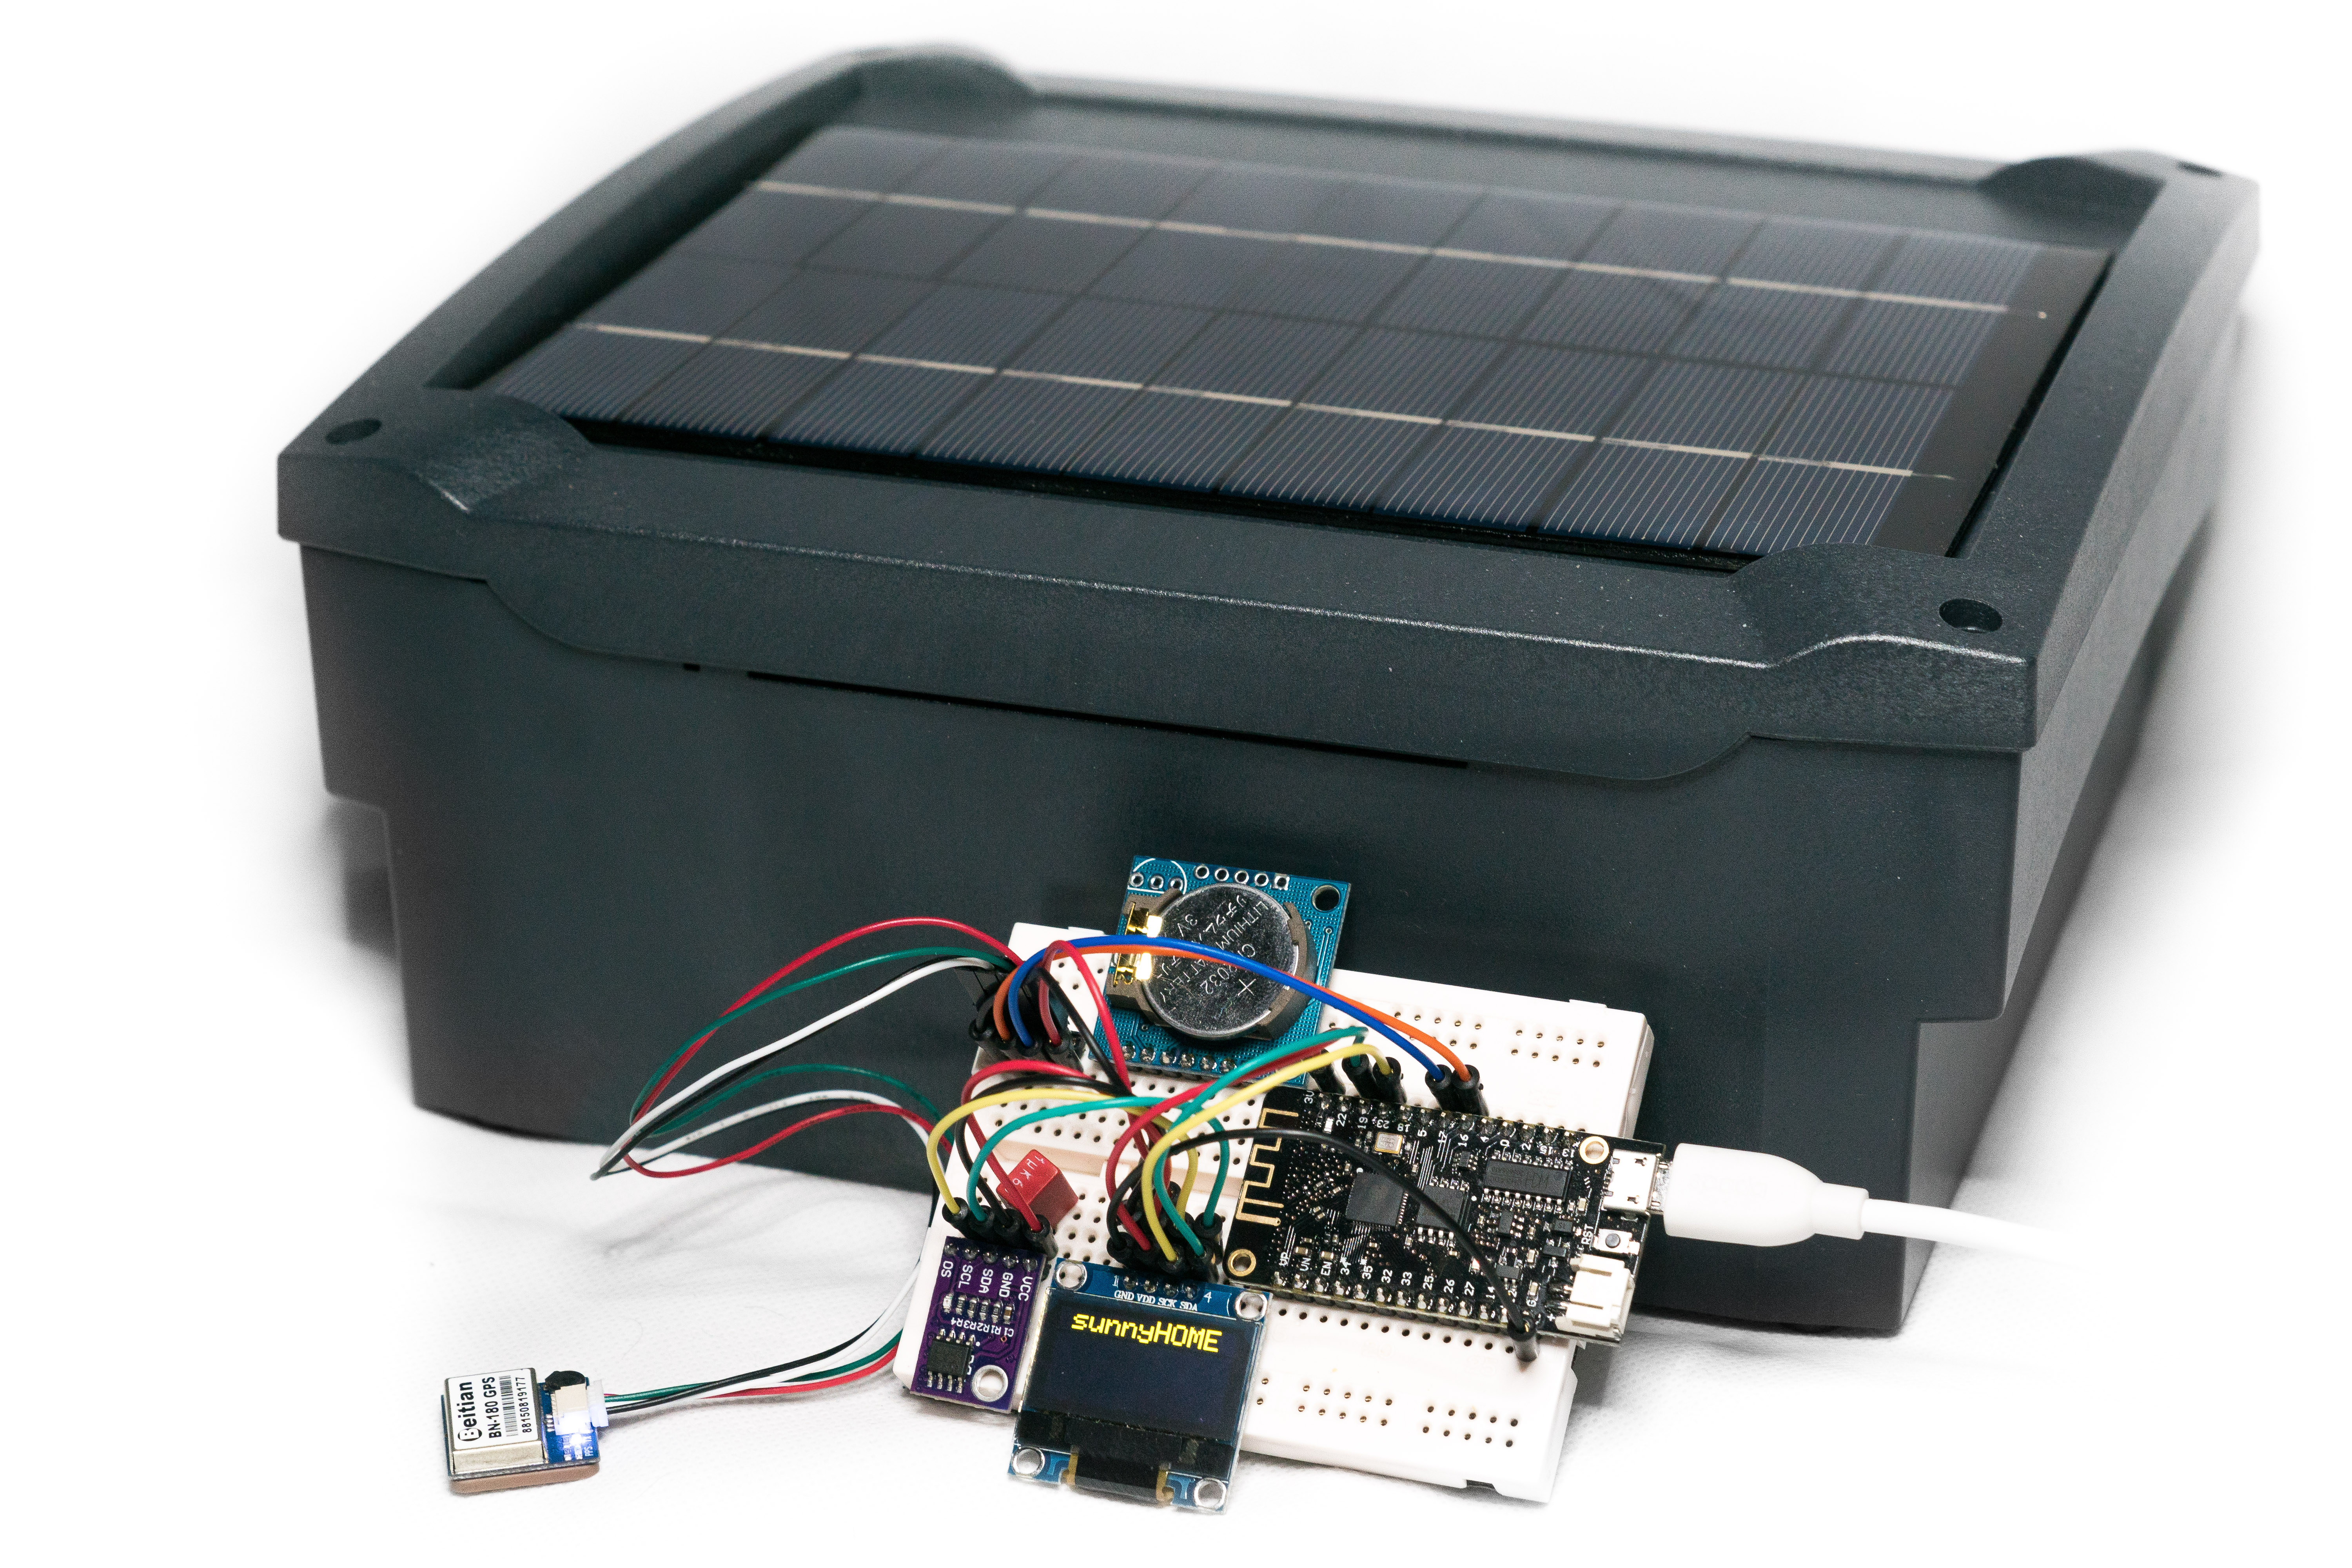
\includegraphics[width=1\linewidth]{media/images/sunnyHOME.jpg}
\end{center}
} \\


\textbf{\mbox{Möglichkeiten der} Einsichtnahme \mbox{in die Arbeit}} & 
{Archiv der HTL Braunau, bzw.\newline \url{https://diplomarbeiten.berufsbildendeschulen.at/}} \\


\end{tabularx}




%--------------------------------------------------------------------------------
% Unterschriften
%--------------------------------------------------------------------------------


\vspace*{\fill}

\textbf{Approbation (Datum / Unterschrift)}

\fbox{
\begin{minipage}[t][3cm]{0.5\linewidth}
Prüfer/Prüferin: \\
%\hspace*{\fill}\includegraphics[width=0.8\linewidth]{fig/Unterschrift}\hspace*{\fill}
\vfill
\end{minipage}}
\fbox{
\begin{minipage}[t][3cm]{0.5\linewidth}
Direktor/Direktorin
\\ Abteilungsvorstand/Abteilungsvorständin
\vfill
\end{minipage}
}

%--------------------------------------------------------------------------------


%--------------------------------------------------------------------------------
%  Vorgeschriebene Dokumentationsseiten (Englisch)
%--------------------------------------------------------------------------------

\pagebreak
\thispagestyle{empty}
\newgeometry{top=2cm, bottom=1.5cm}

\begin{minipage}[c]{0.20\linewidth}
\includegraphics[width=0.8\linewidth]{media/images/htl_c_cmyk_rein}
\end{minipage}
\begin{minipage}[c]{0.6\linewidth}
\begin{center}
{\bfseries\sffamily\large HTBLA Braunau/Inn\\
COLLEGE of ENGINEERING\\
Dept. Elektronik und Technische Informatik\\
{\normalsize Educational focus Communications} }
\end{center}
\end{minipage}
\begin{minipage}[c]{0.2\linewidth}
\hfill \includegraphics[width=0.8\linewidth]{media/images/htl-bildung-mit-zukunft}
\end{minipage}\\

\vspace{1em}
\begin{center}
\bfseries\sffamily\Large
DIPLOMA THESIS Documentation
\end{center}
\vspace{1ex}

\renewcommand{\arraystretch}{2}
\begin{tabularx}{1\textwidth}{ p{3.5cm} X }

\textbf{Author(s)} & 
Andreas Herz \\


\textbf{Form \mbox{Academic year}} & 
5BHELS 2018/2019 \\

\textbf{Topic} & 
\htlArbeitsthema \\

\textbf{Assignment \mbox{of tasks}} & 
{The major task was to develope a self-sufficient weather station. Various sensors should be used,  like for example rainfall- and UV-sensors. The measured data should be read from the ESP32, and then published to a web-server. The web-server evaluates this data, which then will be visualized via a website or a mobile application.} \\

\textbf{Realisation} & 
{The realisation will happen with help of the ESP32 microcontroller. The ESP32 has the needed energy-efficiancy and can be easily connected to a wide variety of sensors. A GPS-receiver should provide the current location of the weather station, and solar cells should  keep the system self-sufficient.} \\

\textbf{Results} & 
{The most important results should be:
    \begin{itemize}
        \item concept is done
        \item sensors are able to measure
        \item receiving the GPS-signal
        \item transfering of data works
        \item visualization works
        \item power-supply works
        \item diploma thesis is written 
    \end{itemize}} \\

    \end{tabularx}

%--------------------------------------------------------------------------------

\pagebreak
\thispagestyle{empty}
\newgeometry{top=2cm, bottom=1.5cm}


\begin{minipage}[c]{0.20\linewidth}
\includegraphics[width=0.8\linewidth]{media/images/htl_c_cmyk_rein}
\end{minipage}
\begin{minipage}[c]{0.6\linewidth}
\begin{center}
{\bfseries\sffamily\large HTBLA Braunau/Inn\\
COLLEGE of ENGINEERING\\
Dept. Elektronik und Technische Informatik\\
{\normalsize Educational focus Communications} }
\end{center}
\end{minipage}
\begin{minipage}[c]{0.2\linewidth}
\hfill \includegraphics[width=0.8\linewidth]{media/images/htl-bildung-mit-zukunft}
\end{minipage}\\

\vspace{1em}

\renewcommand{\arraystretch}{2}
\begin{tabularx}{1\textwidth}{ p{3.5cm} X }

\textbf{\mbox{Illustrative graph,} \mbox{photo} \mbox{(incl. explanation)}} & 
{
The sunnyHOME weather station:
\begin{center}
	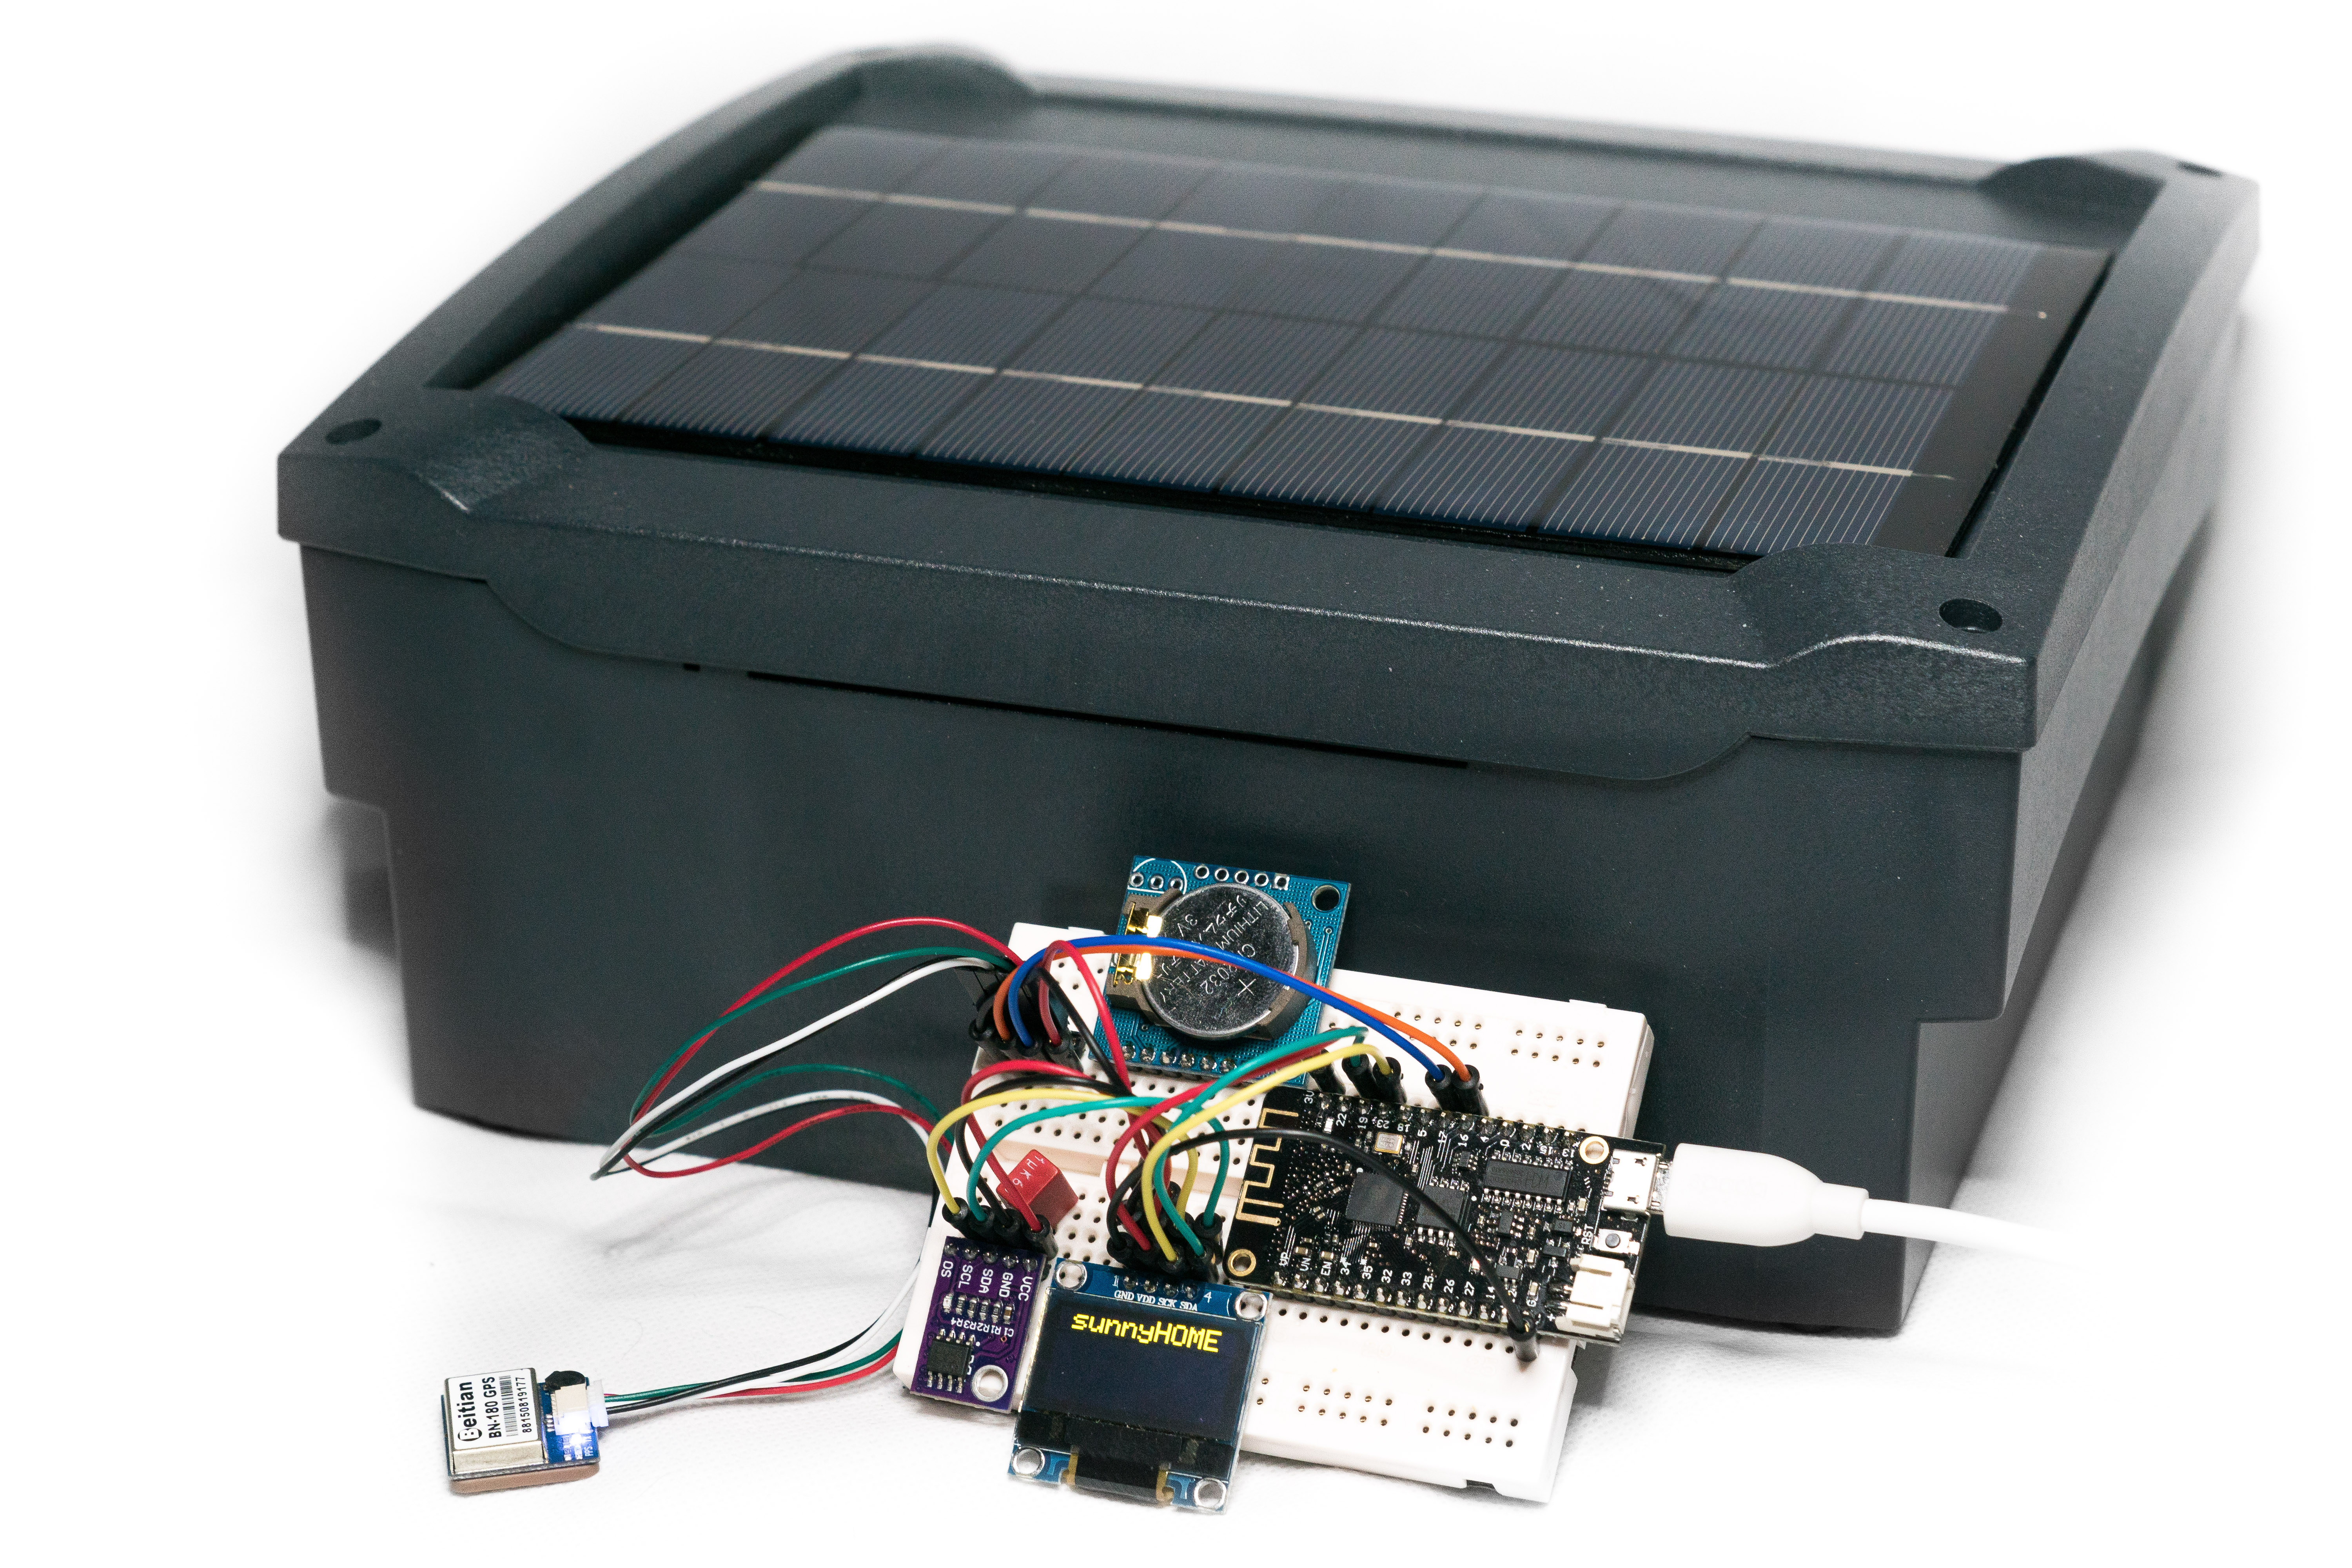
\includegraphics[width=1\linewidth]{media/images/sunnyHOME.jpg}
\end{center}
} \\

\textbf{\mbox{Accessibility of} \mbox{diploma thesis}} & 
{HTL Braunau archive, or\newline \url{https://diplomarbeiten.berufsbildendeschulen.at/}} \\



\end{tabularx}




%--------------------------------------------------------------------------------
% Unterschriften
%--------------------------------------------------------------------------------


\vspace*{\fill}

\textbf{Approval (date / signature)}

\fbox{
\begin{minipage}[t][3cm]{0.5\linewidth}
\centering
Examiner \\
%\hspace*{\fill}\includegraphics[width=0.8\linewidth]{fig/Unterschrift}\hspace*{\fill}
\vfill
\end{minipage}}
\fbox{
\begin{minipage}[t][3cm]{0.5\linewidth}
\centering
Head of College / Department
\vfill
\end{minipage}
}

%--------------------------------------------------------------------------------

\restoregeometry

